\documentclass[a4paper,11pt,spanish,sans]{exam}
\usepackage[spanish]{babel}
%\usepackage[utf8]{inputenc}
\usepackage{multicol}
%\usepackage[latin1]{inputenc}
\usepackage{fontspec}%la posta para las tildes con lualatex
\usepackage[margin=0.5in]{geometry}
\usepackage{amsmath,amssymb}
\usepackage{multicol}
\usepackage{natbib}
\usepackage{graphicx}
\usepackage{hyperref}
\usepackage{epstopdf}
\usepackage{capt-of}
\usepackage{gensymb}
\usepackage{wrapfig}
%\usepackage{animate}
\usepackage[usenames]{color}
\usepackage{tikz}%para graficos
\usetikzlibrary{decorations.markings}
\usetikzlibrary{shapes.geometric}
\usepackage{tkz-euclide}
\usetkzobj{all}

%los de aca abajo capaz no los uso
\newcommand{\class}{Matemática: Guía 2 de  Trigonometria}
\newcommand{\term}{2° Trimestre 2015}
\newcommand{\examnum}{}
\newcommand{\examprof}{Alexis Gomel}
\newcommand{\examdate}{15/7/2015}
\newcommand{\timelimit}{60 Minutes}%no lo uso
\newcommand{\webpdf}{https://drive.google.com/file/d/0B2MOYme4kZd-eS0zUFhNQjV6eUE/view?usp=sharing}%no lo uso
\newcommand{\Ts}{\rule{0pt}{2.6ex}}       % Top strut
\newcommand{\Bs}{\rule[-1.2ex]{0pt}{0pt}} % Bottom strut

%el header de las hojas.
\pagestyle{head}
\firstpageheader{}{}{}
\runningheader{\class}{\examnum\ - Pagina \thepage\ de \numpages}{\examdate}
\runningheadrule

\begin{document}

\noindent
\begin{tabular*}{\textwidth}{l @{\extracolsep{\fill}} r @{\extracolsep{6pt}} l}
\textbf{\class} & \textbf{Profesor: \examprof}\\

\textbf{PDF: \href{\webpdf}{\textcolor{blue}{http://tinyurl.com/Trigonometricas}}} %& Teaching Assistant & \makebox[2in]{\hrulefill}
\end{tabular*}\\
\rule[2ex]{\textwidth}{2pt}

%%%%%%%%%%%%%%%%%%%%%%%%%%%%%%%%%%%%%%%%%%%
%Temas: 


{\small Esta guía, es simplemente una guía. \textbf{NO reemplaza ni incluye todo el material que se da en clase}}.

\begin{center}
\section*{Guía 2 de Funciones Trigonométricas}
\end{center}


Las funciones trigonométricas son aquellas en las que el argumento de la función ('$x$') es un angulo.

Vamos a ver que esta familia de funciones son muy importantes en la geometría y para describir muchas cosas.%arreglar esto.


\section*{Gráficos de funciones trigonométricas}

la formula general del seno como función de x es: 

Empezando por le seno y el coseno:
\begin{center}
\begin{minipage}{0.3\linewidth}
\[ y=\sin (x) \]
\end{minipage}
\begin{minipage}{0.7\linewidth}
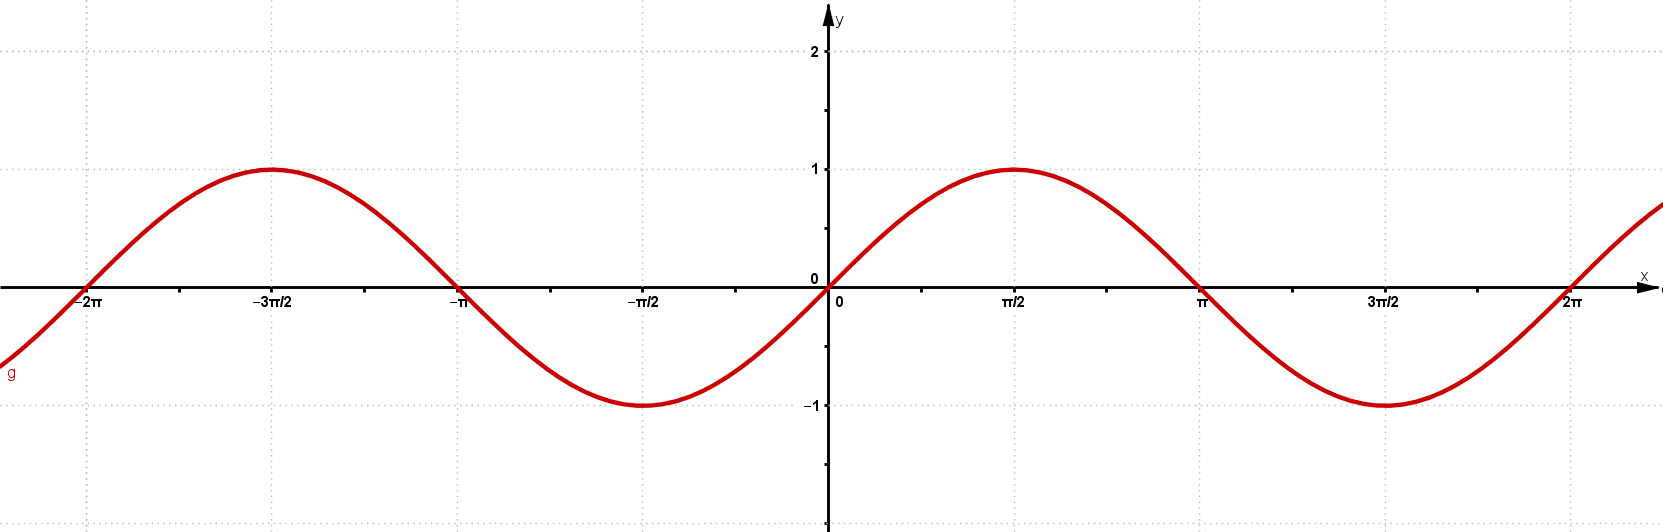
\includegraphics[width=0.5\textwidth]{sin.png}
\end{minipage}

\begin{minipage}{0.3\linewidth}
\[ y=\cos (x)\] 
\end{minipage}
\begin{minipage}{0.7\linewidth}
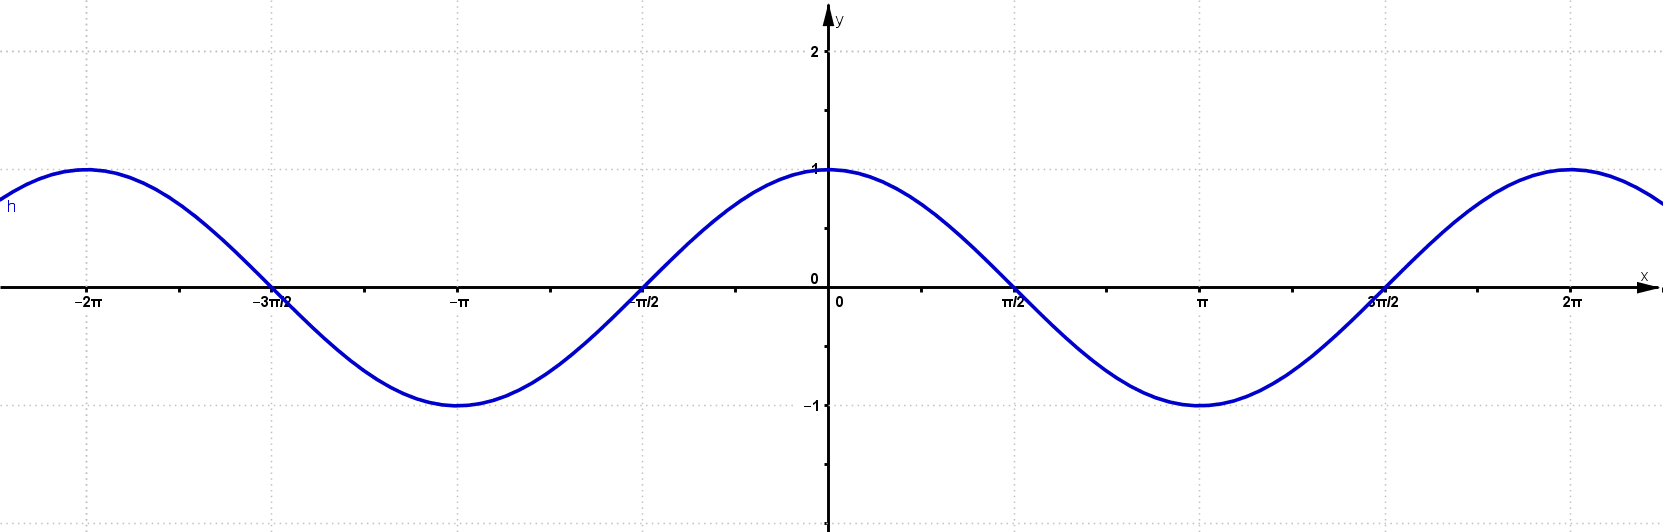
\includegraphics[width=0.5\textwidth]{cos.png}
\end{minipage}

\end{center}

$Dom(\sin (x))= x \in \Re $. Y vale igual para el coseno.

$Im(\sin (x))= [-1,1]$. Y vale igual para el coseno\\

En particular cabe destacar que las funciones trigonométricas se dicen que son $2\pi$ periódicas. ya que toma los mismos valores cada $2\pi$.\\

Una propiedad notoria del seno es que es una función \textbf{Impar}. En el sentido que $\sin(-x)=-\sin(x)$.

Osea que cambia de signo  para los x  negativos, comparado con los positivos.\\

Mientras que el coseno en una función \textbf{par}. En el sentido que $\cos (-x)=\cos (x)$

Osea que es igual tanto para los x positivos como para los negativos.\\

Por otro lado, 

$y=\tan (x)$  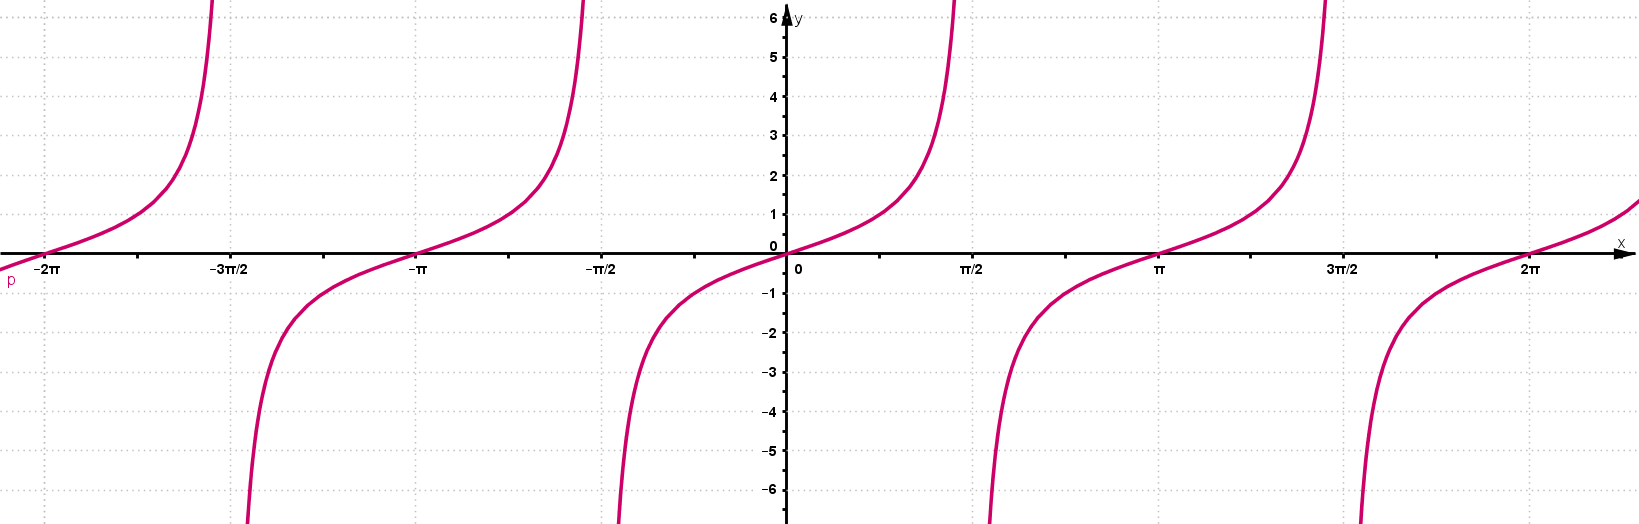
\includegraphics[width=0.5\linewidth]{tan.png}

$Dom(\tan (x))= x \in \Re $. %menos mltiplos de pi/2

$Im(\sin (x))= [-\infty,\infty]$. \\

En general: 

\[
y=A.\sin (w.x + \phi)+D
\]

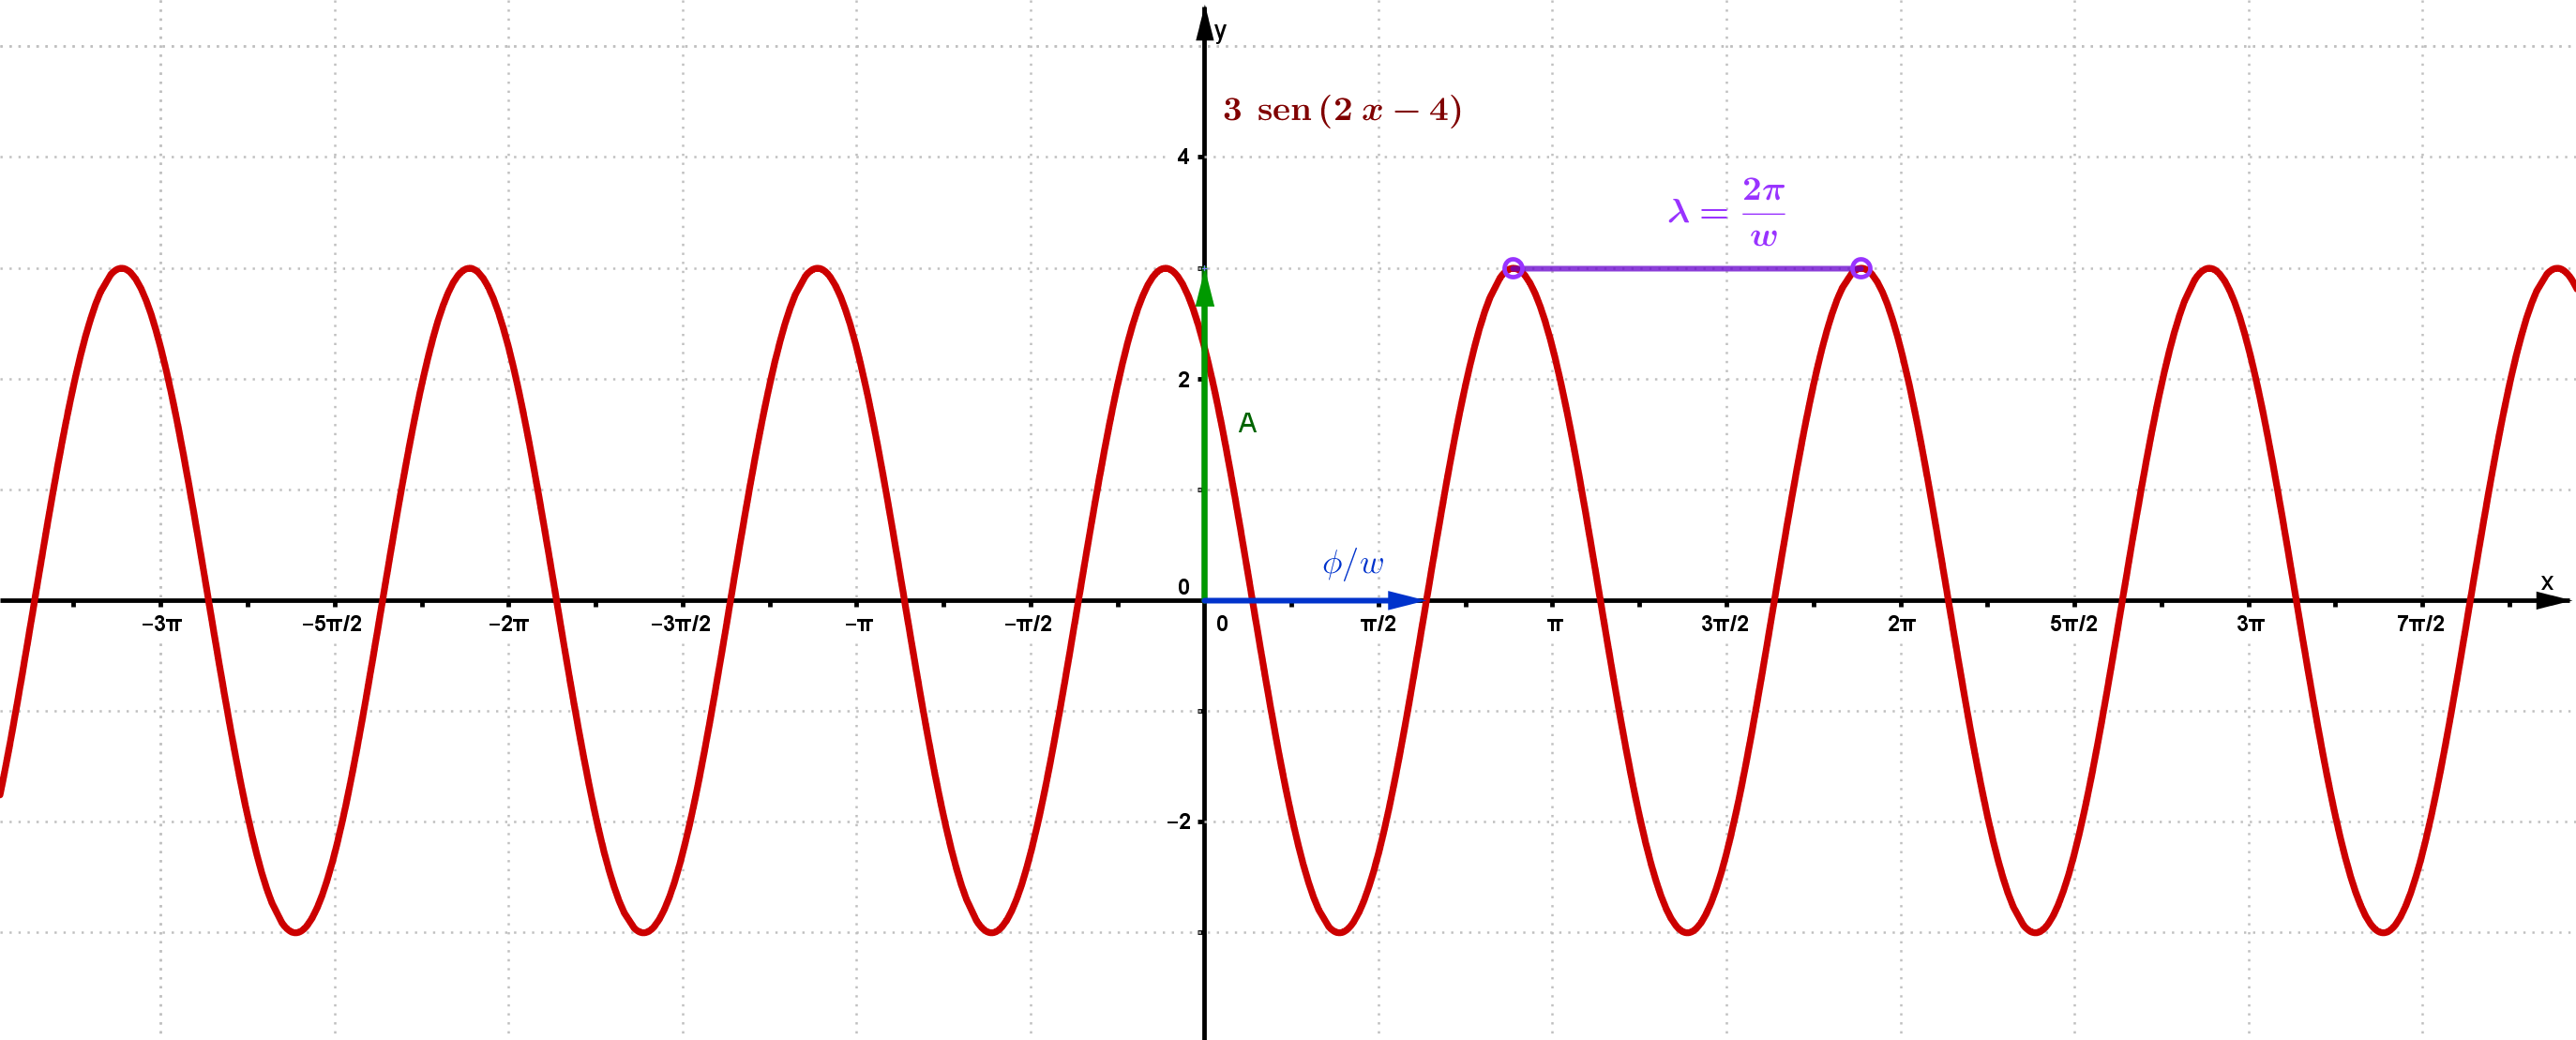
\includegraphics[width=0.5\linewidth]{singeneral.png}
\begin{flushright}
Donde $A$, $w$, $\phi$ y $D$ son constantes.
\end{flushright}

$'A'$ es la amplitud, ya que cambia la amplitud de la oscilación del seno.

\begin{wrapfigure}{r}{0.25\textwidth}
  \begin{center}
    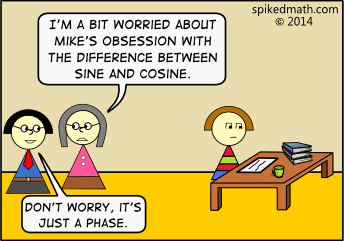
\includegraphics[width=\linewidth]{phase.png}
  \end{center}
\end{wrapfigure}

A $w$ se la llama frecuencia angular, ya que es la que modifica la frecuencia con la que el seno oscila(llega a un máximo, mínimo o pasa por $0$)

A $\phi$ se lo llama fase o corrimiento, y es un factor que corre a la función hacia la izquierda o la derecha.

En particular se puede ver que si $\phi=\frac{w.\pi}{2}$, resulta que $A.\sin (w.x + \phi)=A.\cos(w.x)$.

Osea que el coseno y el seno son la misma función con una fase de diferencia.




\section{Funciones inversas}

Por ultimo, vamos a ver las funciones inversas del seno, el coseno y la tangente.

A una función $g(x)$ se la llama la inversa de $f(x)$, si $f(g(x))=x$. Es decir que si en $f(x)$ uno pone $g(x)$ en lugar de $x$, el resultado de toda la operación vuelve a dar $x$. \\

En este caso a $g(x)$ se la escribe como $f^-1(x)$, que es la notación que se le da a la inversa de la función $f$.\\

Por ejemplo: 

$f(x)= 10^x

g(x)= log(x)

\Rightarrow  f(g(x))= 10^{log(x)}=x    $ y también vale que $g(f(x))=log(10^x)=x$.

En el ejemplo anterior: si $f(x)= 10^x  \Rightarrow f^-1(x)= log(x)$\\

Uso de las funciones inversas: 

si $f(x)=y \Rightarrow f^-1(f(x))=f^-1(y) \Leftrightarrow x=f^-1(y)$

ejemplo: $10^x=y \Rightarrow log(10^x)=log(y) \Leftrightarrow x=log(y)$

Las funciones inversas me da una forma de 'despejar' x cuando esta adentro de una función.

Inversas de funciones trigonometricas: 



$y=\sin (x) \Rightarrow \arcsin(y)=x $  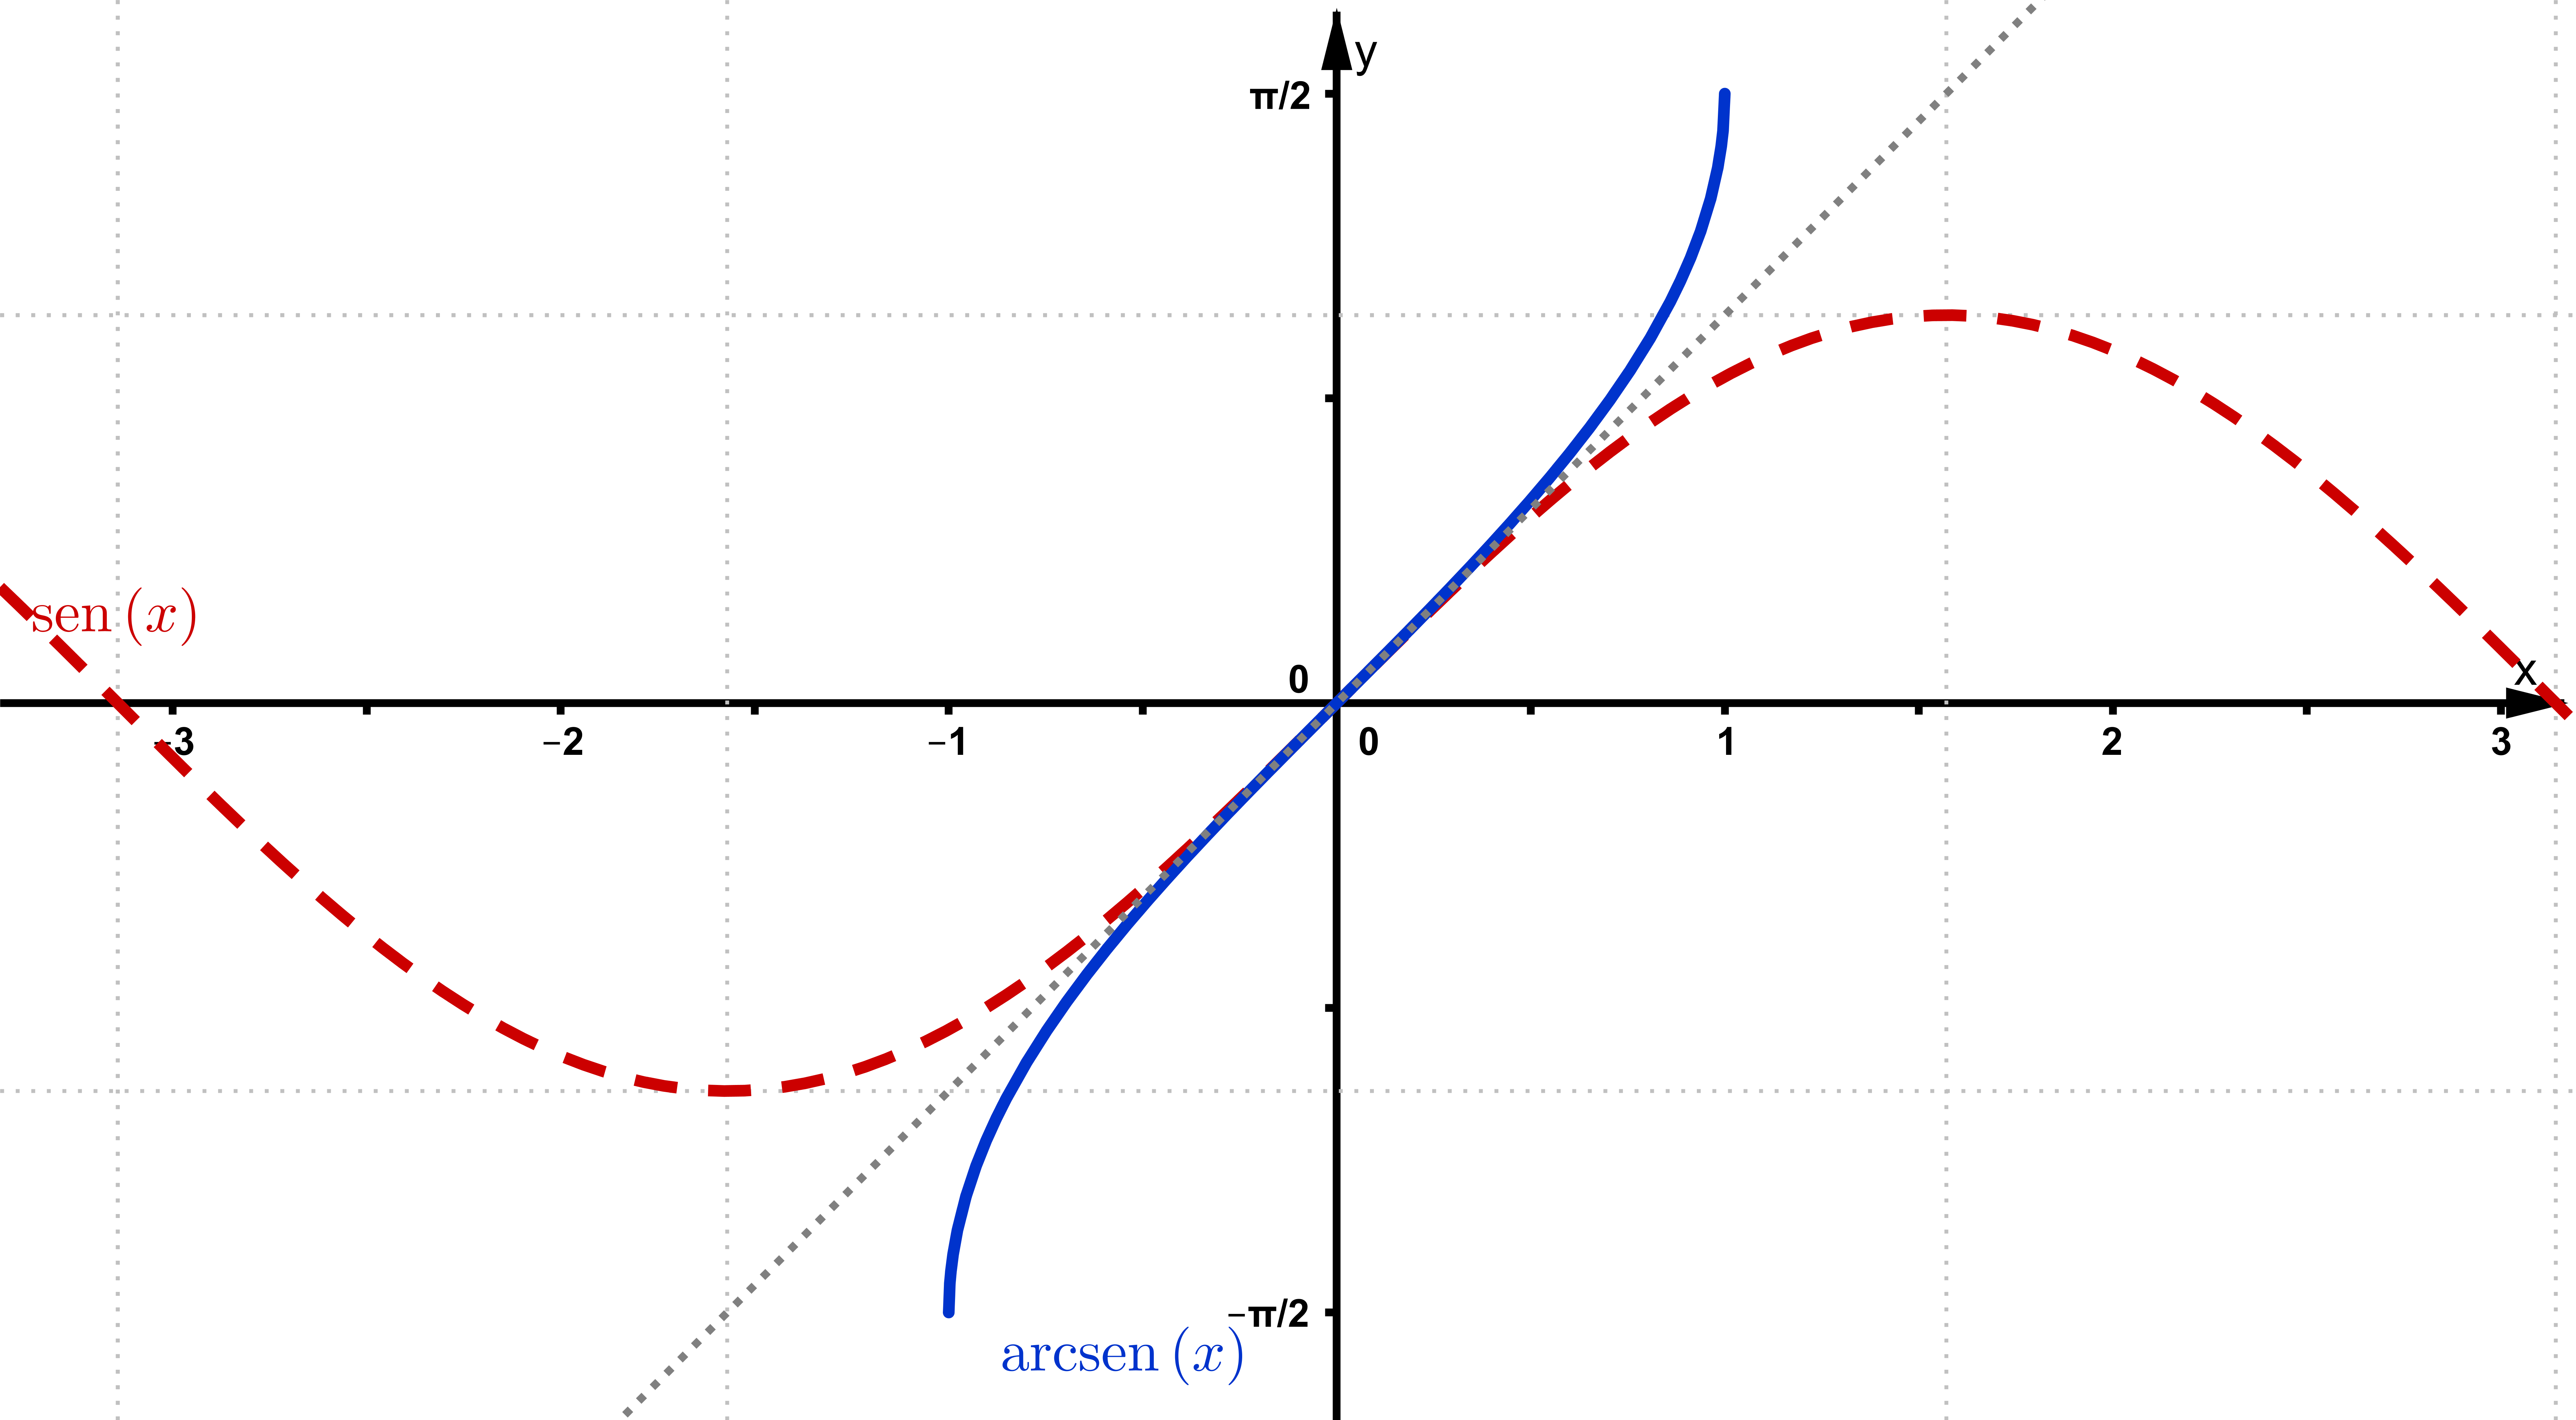
\includegraphics[width=0.5\linewidth]{arcsen.png}
\caption{$y=\sin (x) $ en naranja $y=\arcsin(x)$ en azul. $y=x$ en gris.}

$y=\cos (x) \Rightarrow \arccos(y)=x $  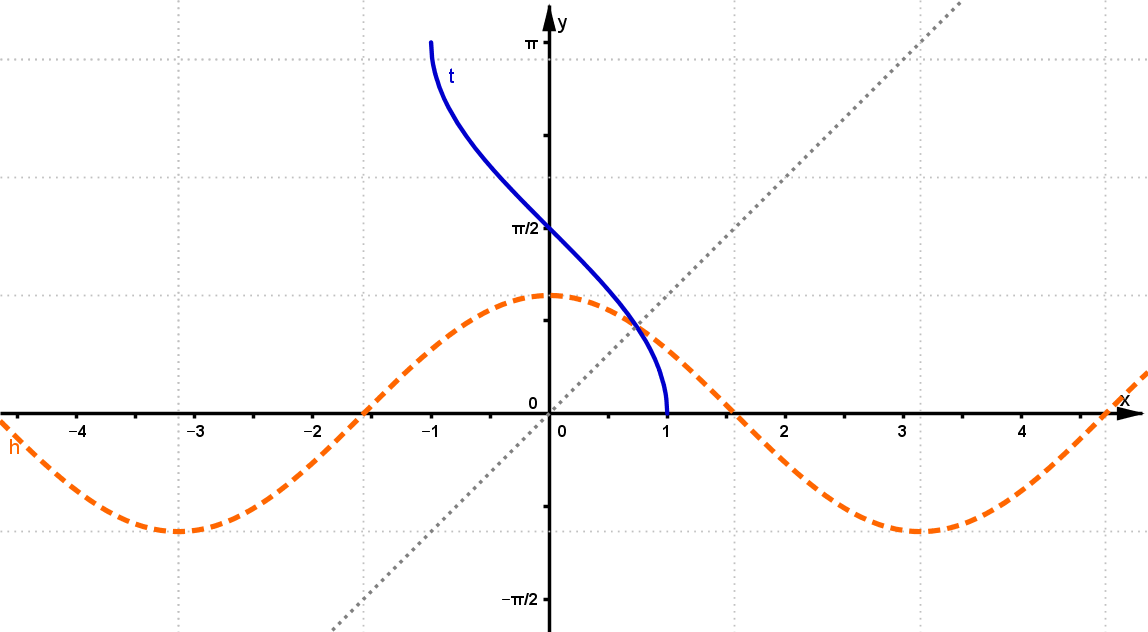
\includegraphics[width=0.5\linewidth]{arccos.png}
\caption{$y=\cos (x) $ en naranja $y=\arccos(x)$ en azul $y=x$ en gris.}

$y=\tan(x) \Rightarrow \arctan(y)=x $  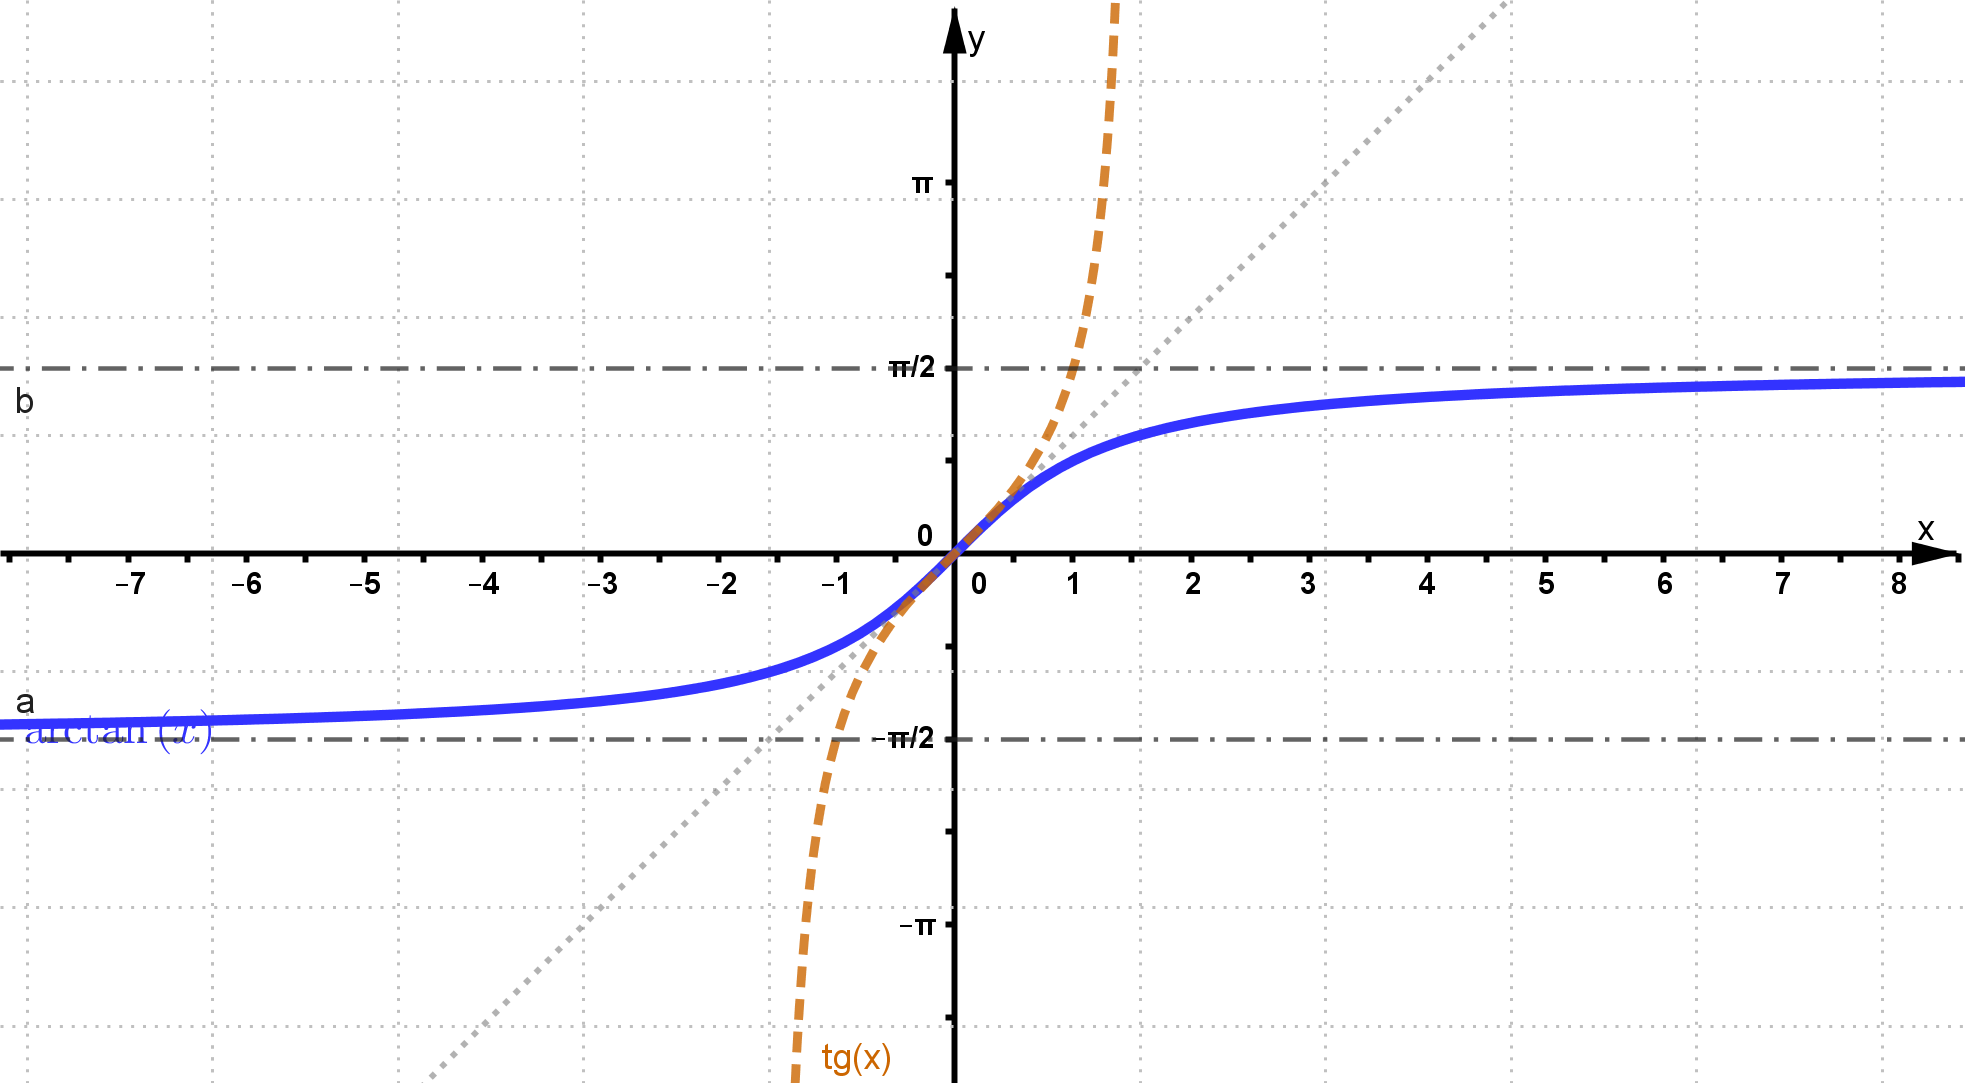
\includegraphics[width=0.5\linewidth]{arctan.png}
\caption{$y=\tan (x) $ en naranja $y=\arctan(x)$ en azul $y=x$ en gris.}

%version ineractiva/gif
%graficos. 

\section*{Relaciones entre las razones trigonométricas.}

Relación Pitagórica:

\[
\sin^2(x)+cos^2(x)=1
\]

Esta es una propiedad muy útil, que vale siempre, sin importar el tipo de  problema.

Otra fácil de deducir es que $\tan(x)=\frac{\sin (x)}{\cos (x)}$.

Hay otra familia de funciones trigonométricas que se derivan a partir de estas tres:

\begin{itemize}
\item  $\cosec (x)=\frac{1}{\sin (x)}$ .  'Cosecante'
\item  $\sec (x)=\frac{1}{\cos (x)}$.  'Secante'
\item  $\cot  (x)=\frac{1}{\tan (x)}=\frac{\cos (x)}{\sin(x)}$ . ' Cotangente'
\end{itemize}


\section*{Ejercicios}

Si se traban con algún ejercicio, pasen al siguiente, y vuelvan al ejercicio difícil mas tarde.

%cosas que voy a buscar: Raices, ordenadas al origen, asintotas. Dom, Im.
%Hacer algun multiple choice.



\section{Gráficos:}
Graficar Las siguientes funciones (basta con usar solo 4 puntos):

\begin{enumerate}%cambiar funcion %ojo con cuales son asintotas oblicuas

%elegir otro ejemplo, capaz el del examen, asi lo tiene visto.
\item Cual de estos gráficos corresponde a $f(x)=\frac{6x-1}{2x+1}$

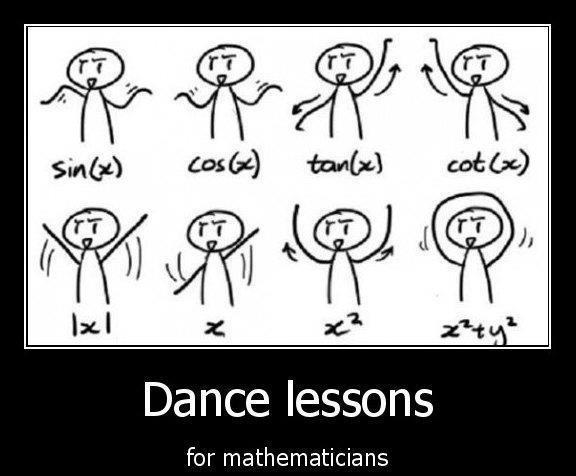
\includegraphics[width=0.2\textwidth]{dance.jpg}
\caption{ }
\label{fig:dance}

\end{enumerate}

\section{Demostrar cada una de las siguientes relaciones entre funciones trigonometricas de un mismo angulo}
\label{demostraciones}

\begin{multicols}{2}%ver restricciones de u

\begin{enumerate}
\item  $ sen^2(u)+cos^2(u)=1 $

\item  $ tg(u)=\frac{sen(u)}{cos(u)} $

\item $cos^2(\alpha)-sen^2(\alpha)=1-2.sen^2(alpha)$

\item $\frac{cos(\alpha)}{cotg(\alpha)}=sen(\alpha)$

\item  $ sen(u).cosec(u)=1 $

\item  $ cos(u).sec(u)=1 $

%poner la suma y resta de cos y sen
\columnbreak 

\item  $ tg(u).cotg(u) $

\item  $ 1+tg^2(u)=\frac{1}{cos^2(u)}=sec^2(u) $

\item  $ 1+cotg^2(u)=\frac{1}{sen^2(u)}=cosec^2(u) $

\end{enumerate}
\end{multicols}

\section{Resolver las ecuaciones}
\label{ecuaciones}

\begin{multicols}{2}%ver restricciones de u

\begin{enumerate}
\item  $ cos^2(x)=cos(x) $

\item $sen(2x)+sen(4x)=0$

%poner la suma y resta de cos y sen
\columnbreak 

\item  $ sen(x)+tg(x)=0 $

\item $4sen^2(x)-8sen(x)+3=0$

\end{enumerate}
\end{multicols}

\section{Ejemplo de Aplicación}

\rule[2ex]{\textwidth}{2pt}

Observación: Para saber si hiciste bien un ejercicio, reemplaza por tu valor de x.

%gifsicle --unoptimize animated.gif | convert - frame-%d.png
%\animategraphics[loop,autoplay]{12}{frame-}{0}{99}
\section*{Extra}

%El numero $e\simeq$ ..  breve bio de euler-
\begin{itemize}
\item Demostración del teorema de pitagoras:

\item Demostración de la relación pitagorica...%%??

\item Toda la geometría que vieron hasta ahora (desde la primaria) cae dentro de una rama de la geometría llamada geometría Eulidea o plana (en honor a Euclides).
Sin embargo existen otros tipos de geometrías, en las cuales pasan cosas a las que no estamos acostumbrados.
Por ejemplo que dos rectas paralelas se toquen, o que la suma  de los ángulos internos de un triangulo sumen mas o menos de 180 grados.
Estas geometrías se llaman geometrías de Riemman o curvas (En honor a Riemman, discípulo de Gauss).

Por ejemplo, dibujar un triangulo que empiece en el polo de la tierra y siga dos latitudes, arma un triangulo cuyos lados internos suman 270 grados.


\end{itemize}

%\bibliographystyle{plain}
%\bibliography{references}

%
%\newpage
%
%\section*{Resultados}
%\begin{enumerate}
%\item
%\begin{enumerate}
%\item -7 ; \item 16 ; \item .. ; \item $3/5$ ; \item 25 ; \item $64/9$ ; \item $c^b $ ;\item $k$ ;\item $\frac{b.d}{c^h} $  ;\item $b=1/c$ ;\item  $2.2,3$ ;\item $2-2,3 = 0,3$ ;\item 2,3/2 ;\item  4,6 ;\item 1$/2,3$ ;\item m/n ;\item  ; 
%\end{enumerate}
%
%\item 
%\begin{enumerate}
%\item
%\item
%\item $log_3(x+1)$
%\end{enumerate}
%
%\item
%\begin{enumerate}
%\item $x=8$
%\item $-2/3$
%\item $x=5$
%\item $x=9$
%\item 
%\item 
%\item $x=2$
%\item $x=2$
%\item $x=1$,$x=$ 
%\end{enumerate}
%
%\item
%
%\item 
%
%
%\end{enumerate}

\end{document}